\subsection{Architectures}
    \paragraph*{}
    Dans un premier temps, je parlerai de l'architecture globale du projet. Puis dans une seconde partie, je parlerai plus précisément de l'architecture du point de vue du drone en terme de communications et de protocoles utilisés.

    \subsubsection{Architecture globale du projet}
        \paragraph*{}
        La figure \ref{fig:archiGen} représente l'architecture générale du projet avec les différents composants utilisés, les connexions entre les composants et les protocoles de communications utilisés. Cette figure représente le projet d'un point de vue très général. J'aborderai dans la partie \ref{part:archiDrone} la partie spécifique au drone et sa communication avec les autres composants du projet.
        
        \paragraph*{}
        L'ordinateur Client communique avec la plateforme via le protocole de communication ModBus. L'application Java est exécutée sur le client et accède en lecture et écriture à la base de donnée intégrée également au client. Le drone accède à la base de données en WiFi et se positionne grâce à des cartes Decawaves utilisant le protocole $UWB$. Le Raspberry Pi connecté sur l'$UART$ du drone permet la communication entre le $SDK$ du drone et le système entier, ce qui permet de faire gérer le déplacement du drone de manière automatisée entre un point de départ et un point d'arrivée qui peut correspondre à un capteur défectueux sur la plateforme ou sur lequel une anomalie a été détectée.
        
        
        Le protocole $UWB$ se définit par une technologie radio pouvant utiliser un très faible niveau d'énergie. Le rayon d'action est de courte portée. Les applications traditionelles de l'$UWB$ sont l'image radar, la collecte de données de capteurs, la localisation et des applications de suivi. La prise en charge de l'$UWB$ a commencé à apparaitre que très récemment dans les Smartphones haut de gamme comme l'iPhone 11 ou le Samsung Galaxy Note20 Ultra, et les AirTag d'Apple. La bande de fréquence d'utilisation commence vers 3.1GHz et va jusqu'à 10.6GHz et ne gêne théoriquement pas les autres communications situées dans ces même bandes.
        
        \begin{figure}[H]
            \centering
        	\begin{frame}{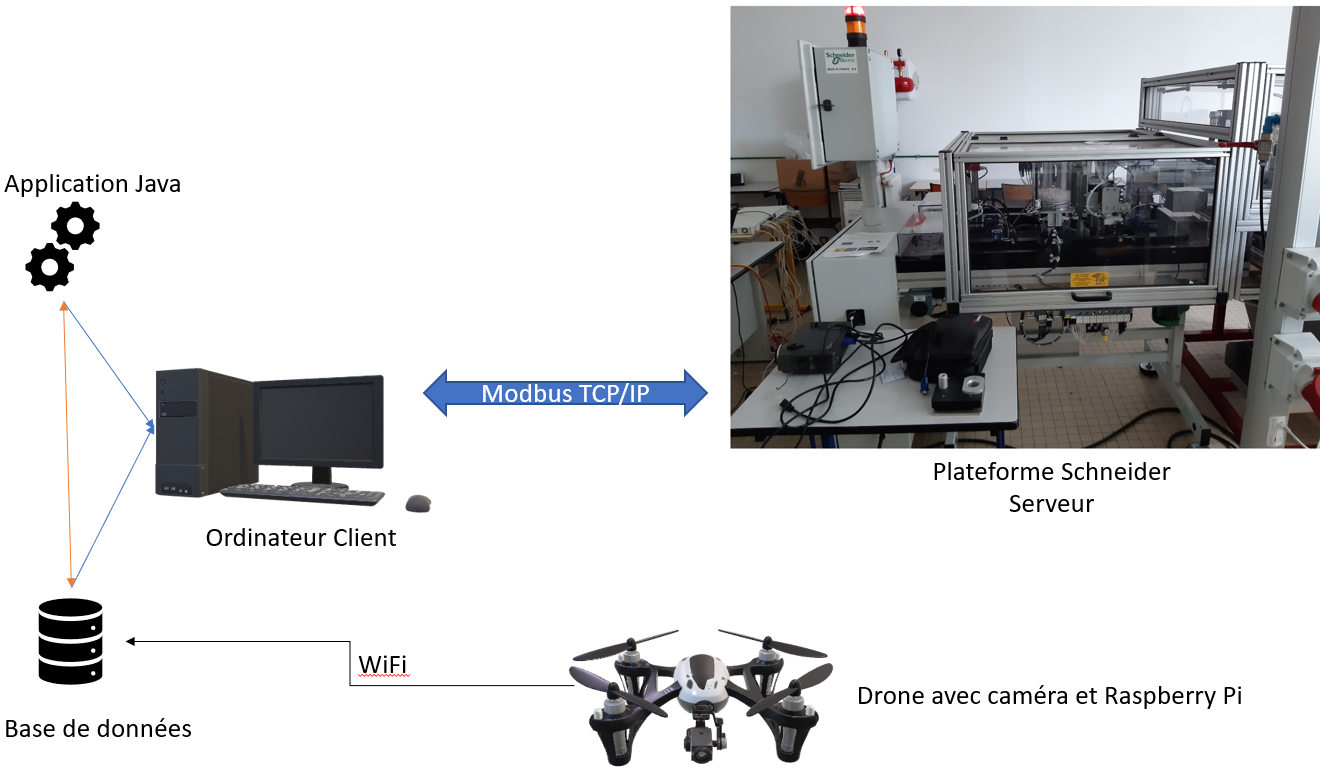
\includegraphics[width=1\textwidth]{image/architectureGenerale.png}}
        	\end{frame}
        	\caption{\label{fig:archiGen}Architecture Générale du projet}
        \end{figure}
    
    \subsubsection{Architecture de la partie drone et explication des communications présentes}
    \label{part:archiDrone}
        \paragraph*{}
        A présent, la figure \ref{fig:archiDrone} correspond à la partie du drone avec le Raspberry Pi 3 B+ lié au drone via une connexion $UART$ (pin 8 et 10 (RX/TX) du Raspberry Pi : voir figure \ref{fig:gpioRPi} pour plus de détails). Par ailleurs, une carte Decawave est connectée sur le Raspberry Pi afin de pouvoir se positionner dans la pièce en communiquant avec 4 autres cartes placées dans la pièce en utilisant une communication $UWB$.
        
        \begin{figure}[H]
            \centering
        	\begin{frame}{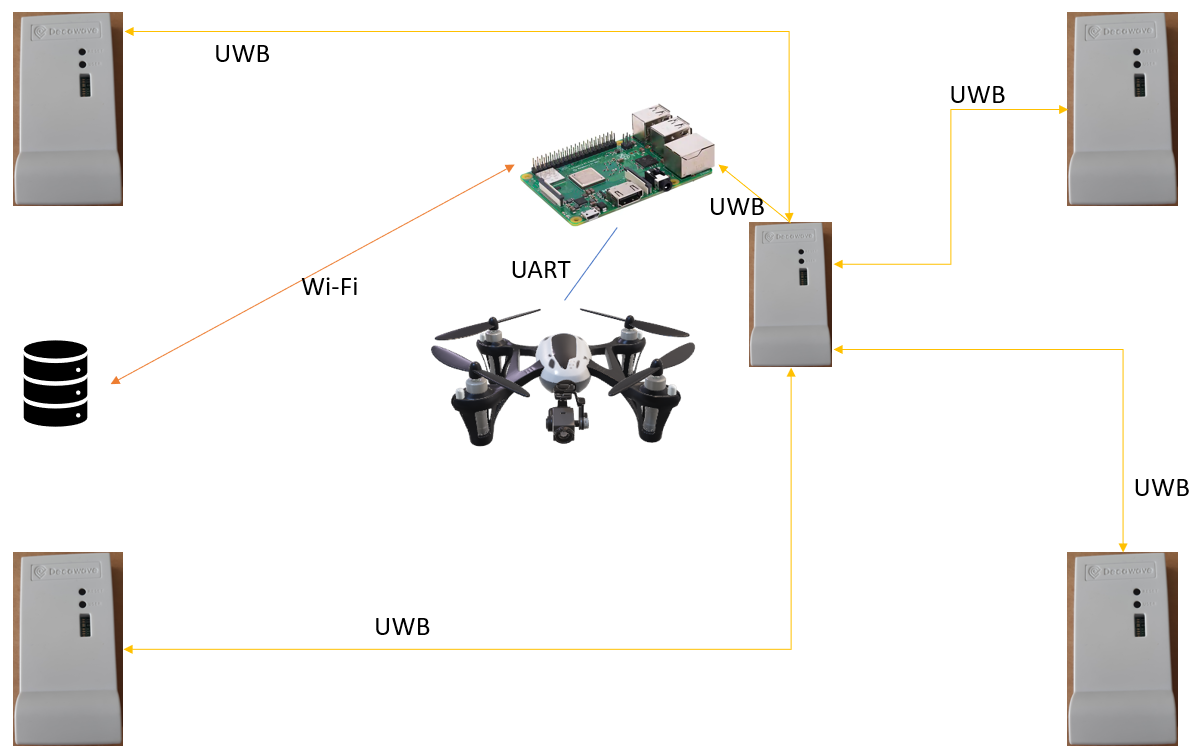
\includegraphics[width=1\textwidth]{image/architectureDrone.png}}
        	\end{frame}
        	\caption{\label{fig:archiDrone}Architecture Drone/Raspberry Pi}
        \end{figure}
        
        \paragraph*{}
        La connexion $UART$\cite{uart} correspond à une connexion entre le Raspberry Pi et le port série du drone. La vitesse de transmission de ce port série est de 230400 bauds dans mon cas afin d'utiliser le Raspberry Pi et le $SDK$ du drone.
        
        \paragraph*{}
        Un trame $UART$ est composé de deux paramètres.
        
        Le premier paramètre est un chiffre correspondant au nombre de bauds\cite{baud}. C'est à dire la vitesse de transmission, un baud représente la fréquence de (dé)modulation d'un signal, c'est-à-dire le nombre de fois où ce signal change par seconde. Il peut être égal au nombre de bit transmis par seconde si l'on considère à tort que la vitesse de transmission et le taux de transfert équivalent à la même chose.
        
        Le second paramètre est composé de trois sous-paramètres. Ils se décomposent en un chiffre, une lettre (I, P, N) et un autre chiffre. Le premier chiffre correspond au nombre de bits de données. La lettre correspond au bit de parité :
        
        \begin{itemize}
            \item[P : ] Parité paire
            \item[I : ] Parité impaire
            \item[N : ] Pas de parité 
        \end{itemize}
        
        Enfin, le troisième sous-paramètre correspond à la durée du bit stop. La durée varie entre 1, 1.5 ou 2.
        
        \begin{figure}[H]
            \centering
        	\begin{frame}{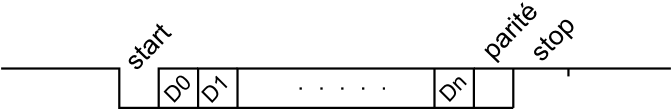
\includegraphics[width=1\textwidth]{image/trame_uart.png}}
        	\end{frame}
        	\caption{\label{fig:trameUART}Exemple d'une trame $UART$}
        \end{figure}
        
        \paragraph*{}
        Voici quelques exemples de paramétrage d'$UART$ :
        
        \begin{itemize}
            \item 4800 4P1 (EN "4800 4E1") : 4800 bauds, 4 bits de données, parité paire (P)(E comme "even" en anglais), 1 bit de stop.
            \item 9600 7I2 (EN "9600 7O2") : 9600 bauds, 7 bits de données, parité impaire (I)(O comme "odd"), 2 bits de stop.
            \item 115200 8N1 : 115200 bauds, 8 bits de données, pas de parité (N), 1 bit de stop.
        \end{itemize}
    
        \paragraph*{}
        Le Raspberry Pi communique avec les cartes Decawaves afin de se positionner dans la pièce. Les cartes qui sont utilisées dans ce stage sont les cartes \textit{MDEK1001}\cite{mdek}. Le protocole de communication utilisé par ces cartes est l'Ultra Large Bande ou Ultra WideBand ($UWB$). Une carte Decawave est relié au Raspberry Pi via USB. Ils communiquent par le port USB en liaison série avec une vitesse de transmission de 115200 bauds. Il y a 4 autres cartes connectées et actives dans la pièce. Il existe deux types de cartes, les ancres qui correspondent à des cartes immobiles dont on connait la position car elle sera fixée par l'utilisateur grâce à l'application Android/iOS fournie par Decawave\cite{androidAppliMdek} et les tags qui correspondent aux cartes mobiles.